\documentclass[10pt]{standalone}
\usepackage[utf8]{inputenc}
\usepackage{pgfplots}
\pgfplotsset{compat=1.15}
\usepackage{mathrsfs}
\usetikzlibrary{arrows}
\pagestyle{empty}
\begin{document}
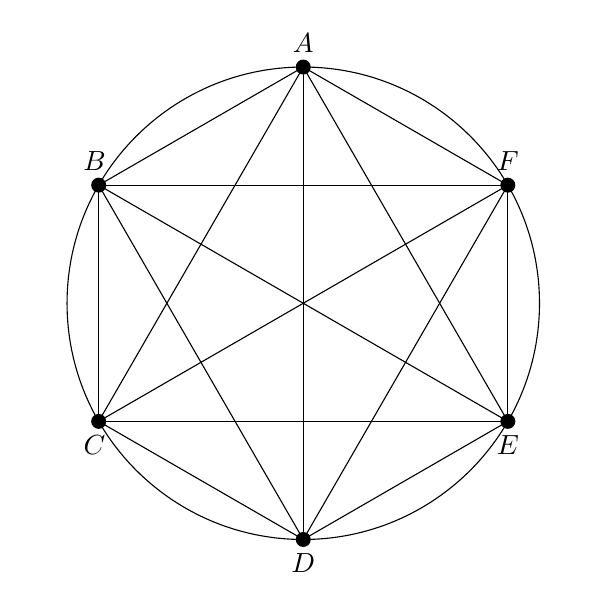
\begin{tikzpicture}[line cap=round,line join=round,>=triangle 45,x=1.0cm,y=1.0cm]
\clip(-0.5,-3.5) rectangle (6.5,3.5);
\draw  (3.,0.) circle (3.cm);
\draw  (3.,3.)-- (0.40192378864668404,1.5);
\draw  (0.40192378864668404,1.5)-- (0.40192378864668404,-1.5);
\draw  (0.40192378864668404,-1.5)-- (3.,-3.);
\draw  (3.,-3.)-- (5.598076211353316,-1.5);
\draw  (5.598076211353316,-1.5)-- (5.598076211353316,1.5);
\draw  (5.598076211353316,1.5)-- (3.,3.);
\draw  (3.,0.)-- (0.40192378864668404,-1.5);
\draw  (3.,0.)-- (3.,-3.);
\draw  (3.,0.)-- (0.40192378864668404,1.5);
\draw  (3.,0.)-- (3.,3.);
\draw  (3.,0.)-- (5.598076211353316,1.5);
\draw  (3.,0.)-- (5.598076211353316,-1.5);
\draw  (3.,3.)-- (0.40192378864668404,-1.5);
\draw  (3.,3.)-- (5.598076211353316,-1.5);
\draw  (5.598076211353316,1.5)-- (3.,-3.);
\draw  (0.40192378864668404,1.5)-- (3.,-3.);
\draw  (0.40192378864668404,1.5)-- (5.598076211353316,1.5);
\draw  (0.40192378864668404,-1.5)-- (5.598076211353316,-1.5);

\draw [fill=black] (3.,3.) circle (2.5pt);
\draw[color=black] (3.0,3.3) node {$A$};
\draw [fill=black] (3.,-3.) circle (2.5pt);
\draw[color=black] (3.0,-3.3) node {$D$};
\draw [fill=black] (5.598076211353316,1.5) circle (2.5pt);
\draw[color=black] (5.6,1.8) node {$F$};
\draw [fill=black] (0.40192378864668404,1.5) circle (2.5pt);
\draw[color=black] (0.35,1.8) node {$B$};
\draw [fill=black] (0.40192378864668404,-1.5) circle (2.5pt);
\draw[color=black] (0.35,-1.8) node {$C$};
\draw [fill=black] (5.598076211353316,-1.5) circle (2.5pt);
\draw[color=black] (5.6,-1.8) node {$E$};
\end{tikzpicture}
\end{document}